%%Cp plots

In this section, we focus on $C_p$ for the different meshes obtained from the zonal-based refinement.
Here, spanwise-averaged data is shown from the second surging cycle (due to limitations on the computational cost).

A comparison of $C_p$ for the different meshes is shown in Figure \ref{fig:zonal_Cp_Re200k_plots}. 
This is done for 4 phases of interest leading up to the LEV formation. 
For $\psi=210^\circ$, $C_p$ for all meshes compares well. Note that for the $Re=40,000$ case, a peak in $C_p$ which indicates LEV formation, was already detected by $\psi=210^\circ$. 

For $\psi=225^\circ$, all meshes show a peak in $C_p$ near the leading edge around $x/c = 0.05$, indicating LEV formation.
Location of this peak in $C_p$ compares well for all meshes.
M0\_nz50, predicts a slightly lower peak value in $C_p$ at this location, as compared to other meshes.

For phase $\psi=240^\circ$, LEV formation can be seen for all the meshes close to the leading edge.
M0\_nz50 mesh predicts a smaller $C_p$ than Mza1\_nz50 and Mza2\_nz50 meshes, which compare well with each other.

At phase $\psi=300^\circ$, TEV formation can be seen for all the meshes close to the trailing edge.
Again, M0\_nz50 mesh predicts a smaller $C_p$ than Mza1\_nz50 and Mza2\_nz50 meshes.
Mza1\_nz50 and Mza2\_nz50 meshes compare well with each other.


\begin{figure}[H]
	\centering
	
	\begin{subfigure}[b]{0.475\textwidth}
		\centering
		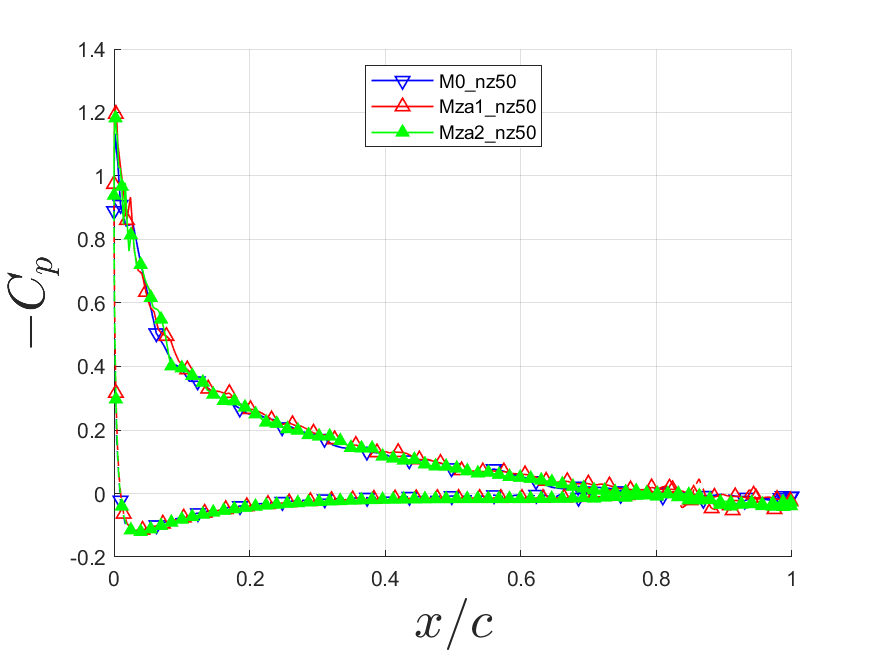
\includegraphics[width=1\textwidth]{figures/zonal_adapt_results/Cp_Re200k/Cp_ph_210.png}
		\caption{ $C_p$ at $\psi$ = $210^\circ$}
		\label{fig:zonal_Cp_Re200k_210}
	\end{subfigure}
	\begin{subfigure}[b]{0.475\textwidth}
	\centering
	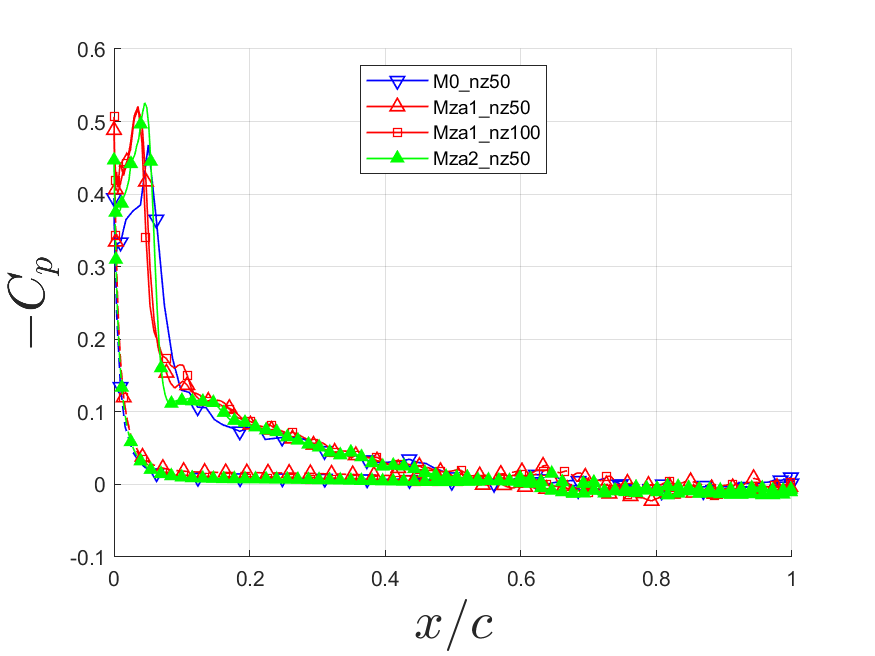
\includegraphics[width=1\textwidth]{figures/zonal_adapt_results/Cp_Re200k/Cp_ph_225.png}
	\caption{ $C_p$ at $\psi$ = $225^\circ$}
	\label{fig:zonal_Cp_Re200k_210}
\end{subfigure}
	\begin{subfigure}[b]{0.475\textwidth}
		\centering
		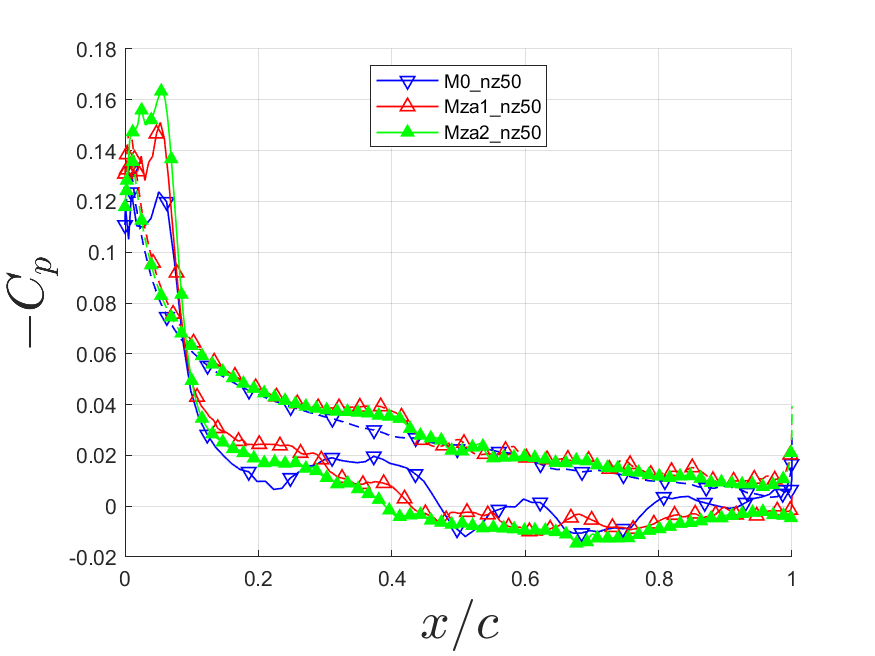
\includegraphics[width=1\textwidth]{figures/zonal_adapt_results/Cp_Re200k/Cp_ph_240.png}
		\caption{ $C_p$ at $\psi$ = $240^\circ$}
		\label{fig:zonal_Cp_Re200k_240}
	\end{subfigure}
	\begin{subfigure}[b]{0.475\textwidth}
	\centering
	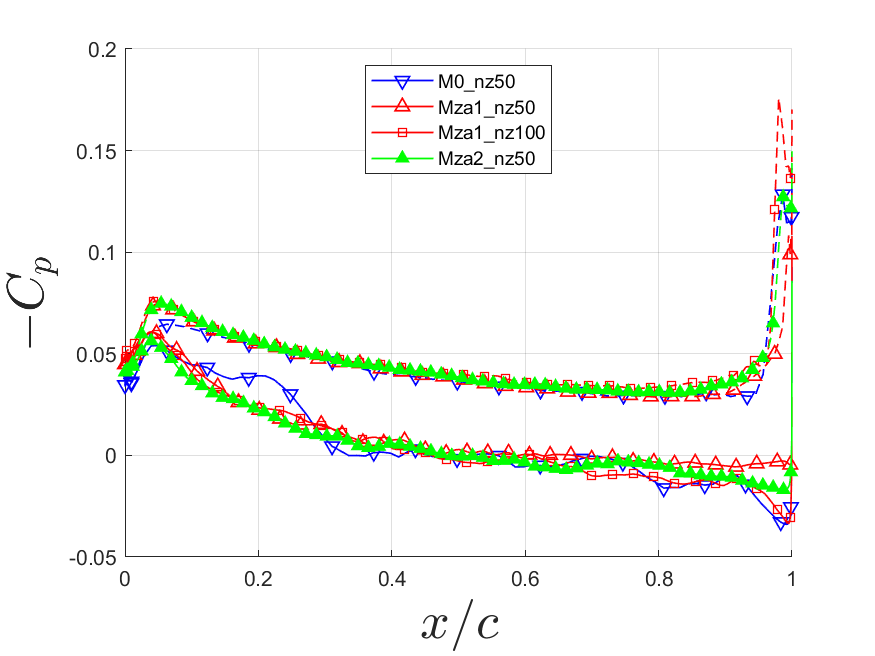
\includegraphics[width=1\textwidth]{figures/zonal_adapt_results/Cp_Re200k/Cp_ph_255.png}
	\caption{ $C_p$ at $\psi$ = $255^\circ$}
	\label{fig:zonal_Cp_Re200k_255}
\end{subfigure}
	\begin{subfigure}[b]{0.475\textwidth}
		\centering
		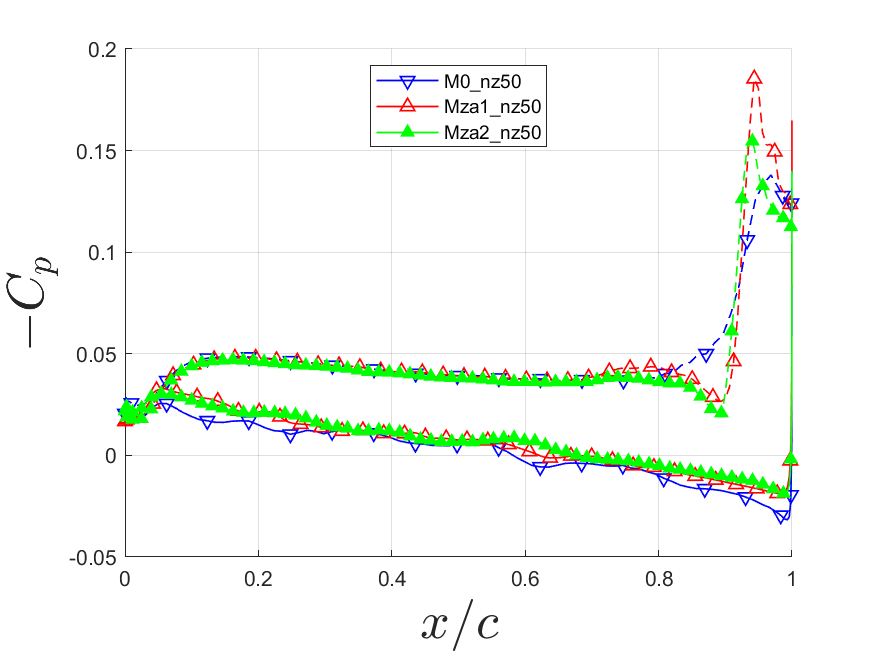
\includegraphics[width=1\textwidth]{figures/zonal_adapt_results/Cp_Re200k/Cp_ph_270.png}
		\caption{ $C_p$ at $\psi$ = $270^\circ$}
		\label{fig:zonal_Cp_Re200k_270}
	\end{subfigure}
	\begin{subfigure}[b]{0.475\textwidth}
		\centering
		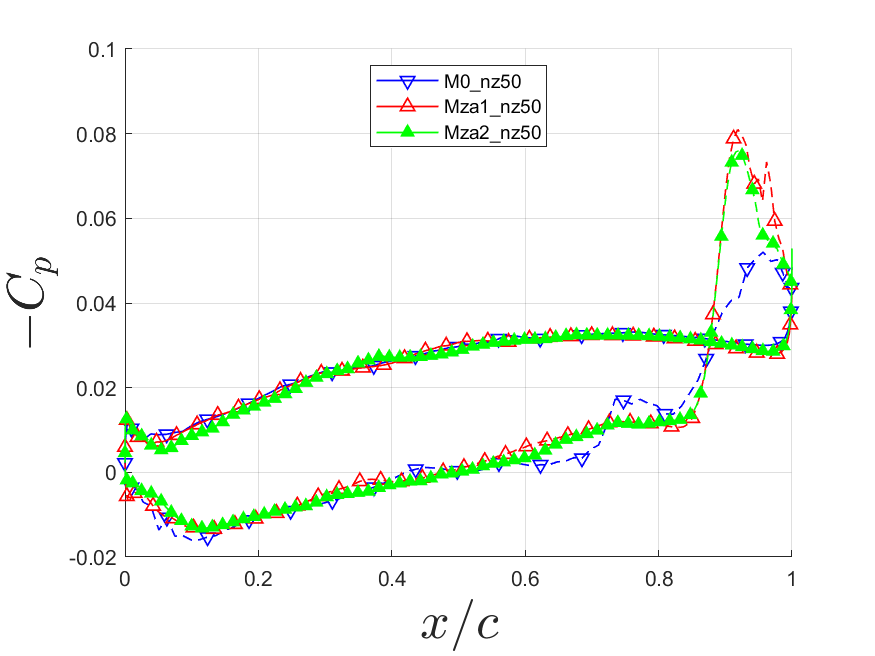
\includegraphics[width=1\textwidth]{figures/zonal_adapt_results/Cp_Re200k/Cp_ph_300.png}
		\caption{ $C_p$ at $\psi$ = $300^\circ$}
		\label{fig:zonal_Cp_Re200k_300}
	\end{subfigure}
	\caption{$C_p$ comparison for different meshes. Top surface $C_p$ is denoted by solid lines and bottom surface $C_p$ is denoted by dashed lines}
	\label{fig:zonal_Cp_Re200k_plots}
\end{figure}